\documentclass{scrartcl}

%%%%%%%%%%%%%%%%%%%%%%%%%%%%%%
\usepackage{hyperref}
\usepackage[pdftex]{graphicx}
\usepackage[usenames]{xcolor}
\usepackage{amssymb}
\usepackage{amsmath}
\usepackage{amsfonts}
\usepackage{listings}
\newcommand{\Iff}{{\tt IFF}}
\newcommand{\nlc}{{\tt NLC}}
\newcommand{\cir}{{\tt CIR}}
\newcommand{\lcr}{{\tt LCR}}
\newcommand{\nms}{{\tt NMS}}
\newcommand{\sbn}{{\tt SBN}}
\newcommand{\ord}{{\tt ORD}}
\newcommand{\dem}{{\tt DEM}}
\newcommand{\nl}{{\tt \backslash n}}
\newcommand{\oct}{{\tt Octave}}
\newcommand{\mylink}[2]{\hyperlink{#1}{#2}}
\newcommand{\mylisting}[1]{\hypertarget{listing:#1}%
{{\sffamily\bfseries\large file : #1 \normalfont}}%
\null\lstinputlisting[]{#1}}
\newcommand{\mylistingm}[1]{\hypertarget{listing:#1.m}%
{{\sffamily\bfseries\large file : #1.m \normalfont}}%
\null\lstinputlisting[]{#1.m_in}}

%%%%%%%%%%%%%%%%%%%%%%%%%%%%%%
\title{IFF version 0.1b1 File Format Specification}
\author{Carlo de Falco}

\begin{document}
\maketitle

\section*{Introduction}

This document contains the specification of an {\bf I}ntermediate 
{\bf F}ile {\bf F}ormat ({\Iff}) for describing coupled electrical circuits, 
devices and systems.
The present version of this documents refers to the {\Iff} version 0.1b1.

%%%%%%%%%%%%%%%%%%%%%%%%%%%%%%
\subsection{List of Files}
A circuit description is comprised of a set of files of three different types:
\begin{itemize}
\item  1 {\cir} ({\bf Cir}cuit) file: an {\tt ASCII } text file with filename 
{$<$circuitname$>$.cir} 
\item  1 {\nms} ({\bf N}a{\bf m}e{\bf s}) file: an {\tt ASCII } text file with 
filename {$<$circuitname$>$.nms} 
\item  $N \geq 1$ {\sbn} ({\bf S}u{\bf bn}et) files: a set of M-functions or 
DLD-functions following the template described in \autoref{ssecsbn} below. 
%\item  1 {\ord} (Re{\bf ord}ering ) file: an M-function or DLD-function 
%following the template described in \autoref{ssecord} below. 
\end{itemize}
{\sbn} files are not necessarily specific to one circuit and can be grouped in 
\emph{libraries} as long as the directory containing the library is added to 
the path when the 
{\Iff} parser is run.

%%%%%%%%%%%%%%%%%%%%%%%%%%%%%%
\subsection{File Formats}
Below we describe the purpose and the syntax of each of file categories.
%%%%%%%%%%%%%%%%%%%%%%%%%%%%%%
\subsubsection{{\cir} files}
The {\cir} file is divided into two sections describing the linear 
time--independent ({\lcr} = {\bf l}inear {\bf c}i{\bf r}cuit) and the 
non--linear and/or time--dependent  ({\nlc} = {\bf n}on--{\bf l}inear 
{\bf c}ircuit) partitions of the circuit respectively. 
The syntax for the {\lcr} and {\nlc} section is identical. 
{\nlc} can also contain linear elements, in fact the whole circuit could be 
described only by the {\nlc} 
section but this could result in the evaluator unnecessarily recomputing local 
matrices for linear 
time--independent elements
The content of {\cir} files is organized as follows\footnote{ This description 
makes use of Extended Backus-Naur Form (EBNF) see this 
\hyperref{http://www.garshol.priv.no/download/text/bnf.html}{}{}{article} 
or the EBNF entry in the \hyperref{http://en.wikipedia.org}{}{}{wikipedia} 
for an explanation of (E)BNF }:

\begin{lstlisting}[language=Mathematica,mathescape=true,backgroundcolor={}]
 cir    := header nlc separator lcr separator ;
 header := '%' version_id '$\nl$' 
           comment* ;
 comment:= '%' text '$\nl$' ;
 nlc    := block* ;
 block  := blockcomment? blockheader pv_matrix vnum_matrix  ;
 block_comment := '%' text '$\nl$' ;
 block_header  := func section n_extvar n_par '$\nl$'  
                  n_rows n_parnames '$\nl$' 
                  par_name*;
 section      :=  string ; 
 n_extvar     :=  number ; 
 n_par        :=  number ; 
 n_rows       :=  number ;
 n_parnames   :=  number ;
 par_name     :=  string ; 
 pv_matrix    :=  matrix ;
 vnum_matrix  :=  matrix ;
 matrix    :=  number+ ; 
 separator := 'END $\nl$' ; 
 lcr       :=  block* ; 
\end{lstlisting}

where

\begin{description}
\item  {\tt version\_id} is a string identifying the version on {\Iff} 
  in which the file is encoded
\item  $\nl$ is the new-line character
\item {\tt string} represents anything that the {\oct} command 
  {\tt s=fscanf(file,\%s) } would parse as a string {\it i.e.} any sequence of 
  chars without white-space
\item {\tt text} is any sequence of chars without a $\nl$, 
  this differs from {\tt string} because it can contain white--space
\item {\tt number} represents anything that the {\oct} command 
  {\tt s=fscanf(file,\%g) } would parse as a number
\item {\tt func} is the name of a function to evaluate the elements 
  described in the block
\item {\tt n\_extvar} Is the number of {\it external variables} 
  for the elements of a block
\item {\tt n\_par} Is the number of {\it parameters} for the elements 
  of a block
\item {\tt n\_rows} Is the number of {\it elements} in a block
\item {\tt n\_parnames} Is the number of {\it parameter names} for the 
  elements of a block, it corresponds to the number of {\tt par\_name} entries.
  If {\tt n\_parnames} is 0 the line with the {\tt par\_name}s is missing.
\item {\tt pv\_matrix} Is a list of {\tt n\_rows} $\times$ 
  {\tt n\_par} numbers separated by any character the 
  {\oct} command {\tt s=fscanf(file,\%g) } would consider whitespace 
  (including $\nl$).
\item [] every row (a set of {\tt n\_par} contiguous entries) 
  in {\tt pv\_matrix} refers to an element of the circuit. 
  The {\tt n\_par} numbers in a row represent the values of the 
  parameters to be passed to the function that evaluates that element.
\item {\tt vnum\_matrix} Is a list of {\tt n\_rows} $\times$ {\tt n\_extvar }
  numbers separated by any character the {\oct} command {\tt s=fscanf(file,\%g) } 
  would consider white-space (including $\nl$).
\item [] every row (a set of {\tt n\_extvar} contiguous entries) 
  in {\tt vnum\_matrix} refers to an element of the circuit. 
  The {\tt n\_extvar} numbers in the row represent the global numbering of the element 
  external variables.
\end{description}

\subsubsection{{\nms} files}

{\nms} files are meant to contain the names of the circuit variables, 
the format of {\nms} is just a list
of variable names one on each row preceded by the variable number:

\begin{lstlisting}[language=Mathematica,mathescape=true,backgroundcolor={}]
nms        :=  version_id '$\nl$' comment* line* ;
line       := var_number var_name ;
var_number := number ;
var_name   :=  string ;
\end{lstlisting}

the variable are ordered as follows:
\begin{itemize}
\item first all external variables of all elements 
in the order given by the global numbering of external variables as 
explicitly written in the {\cir} 
files
\item then the internal variables of the elements in the same order as the
corresponding elements appear in the {\cir} file 
( internal variables of non-linear elements first, then those of linear elements)
\end{itemize}

Notice that the number of internal variables of each element is not included 
in the {\Iff} files. 
This is because elements with a number of internal variables that is huge, that depends on the value of some parameter, or even that changes in time (for example distributed elements treated with a FEM with adaptive meshing, a large linear sub-circuit that is reduce via MOR...) and therefore it is more convenient to compute the number of internal variables when initializing the system.

\subsubsection{{\sbn} files} \label{ssecsbn}

{\sbn} files are {\oct} functions, implemented as (M-scripts or as 
DLD functions) with a header as follows:

\begin{lstlisting}
function [a,b,c,] =...
 func (string, m(i,:), extvar, intvar, t)
\end{lstlisting}

i.e. it should get as inputs:

\begin{itemize}
\item  the string entry of the block header
\item  one row of the {\tt pv\_matrix} entry of the block
\item  the current values of all internal and external variables
\item  the current time
\end{itemize} 

and it should produce as outputs three matrices: 
\begin{itemize}
\item  $a,b \in \mathbb{R}^{
\mbox{\tt (n\_extvar + n\_intvar})\times \mbox{\tt (n\_extvar + n\_intvar)}}$ 
\item $c\in \mathbb{R}^{\mbox{\tt (n\_extvar + n\_intvar)}} $ 
\end{itemize}


where {\tt n\_intvar} is the number of \emph{internal variables} 
(see \autoref{sec:appintext} for explanation of \emph{internal variables} and
 \emph{external variables} )
that can be assembled in the complete system matrices.
We assume that the full DAE system can be written in the form
\begin{equation}\label{eqdaesystem}
\left(A(t) \mathbf{x}\right)_{,t} + 
B \mathbf{x} + \mathbf{C} + \mathbf{f}(\mathbf{x},t)= 0
\end{equation}

The local matrices $a$,$b$,$c$ of a linear element $E_{l}$, 
will contain the contributions to $A$, $B$, $C$  due to
$E_{l}$.

At a given instant of time $t=\tilde{t}$ and for a given set of state 
variables $\mathbf{x}=\mathbf{\tilde{x}}$,
the local matrices of a non-linear element $E_{nl}$, 
will contain the local contributions to:
\begin{itemize}
\item $a$ to $A(\tilde{t})$
\item $b$ to the Jacobian matrix 
$\left.\frac{\partial \mathbf{f}}{\partial\mathbf{x}}\right|_{\mathbf{x}=
  \mathbf{\tilde{x}},t=\tilde{t}}$ 
\item $c$ to $\mathbf{f}(\mathbf{\tilde{x}},\tilde{t})$ 
\end{itemize}
due to $E_{nl}$.


\subsection{Internal and External Variables}\label{sec:appintext}
To better understand what is intended by \emph{internal} and \emph{external}
variables we consider below an example with a linear system,
For another example see~\cite{freund99}, Pag.398.

Consider the system below, where, for sake of simplicity,
we assume all coefficient matrices to be independent of time and
of the state vector $\mathbf{x}$

\begin{equation}\label{eq:coupledlinsys}
S: \,\, A \mathbf{x}_{,t} + B \mathbf{x} + \mathbf{C} = 0.
\end{equation}

We assume that the system $S$ obeying~\eqref{eq:coupledlinsys} can be 
partitioned into two subsystems $S1$ and $S2$ and therefore the state 
vector $\mathbf{x}$ can be written as:
\newcommand{\xprtd}{\left[\begin{array}{c}%
\mathbf{x}_{c} \\
\mathbf{x}_{1} \\
\mathbf{x}_{2} \\
\end{array}\right]}
\begin{equation}\label{eq:staepart}
\mathbf{x} = \xprtd
\end{equation}
where $\mathbf{x}_{1}$ represents the vector of the unknowns belonging only to 
$S1$, $\mathbf{x}_{2}$ represents the vector of the unknowns belonging only to 
$S2$ and $\mathbf{x}_{c}$ represents the vector of the unknowns common to 
$S1$ and $S2$.
If $\mathbf{x}_{1}$ and $\mathbf{x}_{2}$ depend on each other only through 
$\mathbf{x}_{c}$, then the \emph{flat} representation~\eqref{eq:coupledlinsys} 
takes the form

\newcommand{\MTT}[9]{\left[
    \begin{array}{ccc}#1 & #2 & #3 \\#4 & #5 & #6 \\#7 & #8 & #9
    \end{array}
  \right]}

\begin{equation}\label{eq:partitionedcoupledlinsys}
S: \,\,  \MTT{A_{cc1}+A_{cc2}}{A_{c1}}{A_{c2}}
{A_{1c}}{A_{11}}{0}
{A_{2c}}{0}{A_{22}}
\left(\xprtd\right)_{,t} + 
\MTT{B_{cc1}+B_{cc2}}{B_{c1}}{B_{c2}}{B_{1c}}{B_{11}}{0}{B_{2c}}{0}{B_{22}}
\xprtd + \left[
  \begin{array}{c}%
    \mathbf{C}_{c1}+\mathbf{C}_{c2} \\
    \mathbf{C}_{1} \\
    \mathbf{C}_{2} \\
  \end{array}\right]
= 0.
\end{equation}

which is equivalent to

$$
\begin{array}{ll}
(A_{cc1}+A_{cc2}) \mathbf{x}_{c,t} + A_{c1}  \mathbf{x}_{1,t} +
A_{c2}  \mathbf{x}_{2,t} + (B_{cc1}+B_{cc2}) \mathbf{x}_{c} +
B_{c1} \mathbf{x}_{1} + B_{c2} \mathbf{x}_{2} + (C_{c1} + C_{c2}) &= 0\\
%
A_{1c}  \mathbf{x}_{c,t} + A_{11}  \mathbf{x}_{1,t} + 
B_{1c}  \mathbf{x}_{c} + B_{11} \mathbf{x}_{1} + C_{1} &= 0\\
%
A_{2c}  \mathbf{x,t}_{c} + A_{22}  \mathbf{x}_{2,t} + 
B_{2c}  \mathbf{x}_{c} + B_{22} \mathbf{x}_{1} + C_{2} &= 0\\
\end{array}
$$

Then $S$ can be represented as the coupling of two systems $S1$ and $S2$ in 
the following way:

\newcommand {\matrow}[2]{\left[ \begin{array}{cc} #1 & #2 \end{array}\right]}
\newcommand {\matcol}[2]{\left[ \begin{array}{c} #1 \\ #2 \end{array}\right]}

\begin{eqnarray}
\label{eq:s1}
S1 : & & \,\, \matrow{A_{1c}}{A_{11}} \matcol{ \mathbf{x}_{1,t}^{(e)}}{ \mathbf{x}_{1,t}} +  \matrow{B_{1c}}{B_{11}} \matcol{ \mathbf{x}_{1}^{(e)}}{ \mathbf{x}_{1}} + C_{1} = 0 \\
%
\label{eq:s2}
S2 : & &\,\, \matrow{A_{2c}}{A_{22}} \matcol{ \mathbf{x}_{2,t}^{(e)}}
{ \mathbf{x}_{2,t}} +  \matrow{B_{2c}}{B_{22}} 
\matcol{ \mathbf{x}_{2}^{(e)}}{ \mathbf{x}_{2}} + C_{2} = 0 \\
%
\label{eq:s1s2coupling}
COUPLING : & & \,\, 
\left\{\begin{array}{l}
\mathbf{x}_{1}^{(e)} = \mathbf{x}_{2}^{(e)} = \mathbf{x}_{c} \\[.5cm]
\matrow{A_{cc1}}{A_{c1}} 
\matcol{ \mathbf{x}_{1,t}^{(e)}}{ \mathbf{x}_{1,t}} + 
\matrow{A_{cc2}}{A_{c2}} 
\matcol{ \mathbf{x}_{2,t}^{(e)}}{ \mathbf{x}_{2,t}} + \\
+ \matrow{B_{cc1}}{B_{c1}} 
\matcol{ \mathbf{x}_{1}^{(e)}}{ \mathbf{x}_{1}} +
\matrow{B_{cc2}}{B_{c2}} 
\matcol{ \mathbf{x}_{2}^{(e)}}{ \mathbf{x}_{2}} +
C_{c1} + C_{c2} = 0
\end{array}\right.
\end{eqnarray}

It is easy to see that, reversing the procedure shown above, it is possible 
to reconstruct the full system $S$ from the subsystems $S1$ and $S2$ the 
information that is needed for this purpose is the following:

\begin{itemize}
\item the local matrices 
  \begin{eqnarray}
    \label{eq:locmati}
    A_{i} = & &
    \left[ \begin{array}{cc} A_{cci} & A_{ci} \nonumber \\   
        A_{ic} & A_{ii} \end{array}  \right]\\
    B_{i} = & &
    \left[ \begin{array}{cc} B_{cci} & B_{ci} \\   
        B_{ic} & B_{ii} \end{array} \right] \nonumber \\
    C_{i} = & &
    \left[ \begin{array}{c} C_{ci} \\   
        C_{i} \end{array} \right] \nonumber \\
    i=1,2 && \nonumber
  \end{eqnarray}
\item a partitioning of the state variables of each subsystem in 
  \emph{internal} ($\mathbf{x}_{i}$) and \emph{external}
  ($\mathbf{x}_{i}^{(e)}$) variables:
\item a \emph{global numbering} of external variables {\it i.e.} an 
  equation of the form of~\eqref{eq:s1s2coupling} or more generally,
  in the case the ordering of the external variables is different in
  the subsystems, a set of identities of the form 
  $$ x_{i}^{(e)} (j) = x_c (j)$$
\end{itemize}


\subsection{Examples}

In this section a set of examples is provided to show how to represent some
circuit topologies in the {\Iff} format, how to parse {\Iff} files and how
to build the systems of equations to be solved at each linearization step 
within each time-step of a transient simulation.
The programs shown are simplified versions of thos included in the OCS package.

\begin{table}
\begin{tabular}{|p{.15\linewidth}|l|l|l|l|l|}
\hline
description & script & flag & {\cir} file & {\nms} file & {\sbn} file(s) \\
\hline \hline
%%
An inverting amplifier with one n-channel MOSFET and a resistive load &
\mylink{listing:runme.m}{\tt runme.m} &
\mylink{listing:runme.m}{\tt nmos} &
\mylink{listing:nmos.cir}{\tt nmos.cir} &
\mylink{listing:nmos.nms}{\tt nmos.nms} &
\begin{minipage}{.2\linewidth}
\mylink{listing:Mnmosfet.m}{\tt Mnmosfet.m}\\ 
\mylink{listing:Mvoltagesources.m}{\tt Mvoltagesources.m}\\ 
\mylink{listing:Mresistors.m}{\tt Mresistors.m}
\end{minipage}\\ \hline
%%
An inverting amplifier with one p-channel MOSFET and a resistive load &
\mylink{listing:runme.m}{\tt runme.m} &
\mylink{listing:runme.m}{\tt pmos} &
\mylink{listing:pmos.cir}{\tt pmos.cir} &
\mylink{listing:pmos.nms}{\tt pmos.nms} &
\begin{minipage}{.2\linewidth}
\mylink{listing:Mpmosfet.m}{\tt Mpmosfet.m}\\ 
\mylink{listing:Mvoltagesources.m}{\tt Mvoltagesources.m}\\ 
\mylink{listing:Mresistors.m}{\tt Mresistors.m}
\end{minipage}\\ \hline
%%
A CMOS inverter with one n-channel and one p-channel MOSFET &
\mylink{listing:runme.m}{\tt runme.m} &
\mylink{listing:runme.m}{\tt inverter} &
\mylink{listing:inverter.cir}{\tt inverter.cir} &
\mylink{listing:inverter.nms}{\tt inverter.nms} &
\begin{minipage}{.2\linewidth}
\mylink{listing:Mpmosfet.m}{\tt Mpmosfet.m}\\ 
\mylink{listing:Mvoltagesources.m}{\tt Mvoltagesources.m}\\ 
\mylink{listing:Mnmosfet.m}{\tt Mnmosfet.m}
\end{minipage}\\ \hline
%%
A CMOS AND gate with three n-channel and three p-channel MOSFETs &
\mylink{listing:runme.m}{\tt runme.m} &
\mylink{listing:runme.m}{\tt and} &
\mylink{listing:and.cir}{\tt and.cir} &
\mylink{listing:and.nms}{\tt and.nms} &
\begin{minipage}{.2\linewidth}
\mylink{listing:Mpmosfet.m}{\tt Mpmosfet.m}\\ 
\mylink{listing:Mvoltagesources.m}{\tt Mvoltagesources.m}\\ 
\mylink{listing:Mnmosfet.m}{\tt Mnmosfet.m}
\end{minipage}\\ \hline
%%
An inverting amplifier with one n-channel MOSFET and a capacitive load  &
\mylink{listing:runmedaspk.m}{\tt runmedaspk.m} &
\mylink{listing:runmedaspk.m}{\tt nmos2} &
\mylink{listing:nmos2.cir}{\tt nmos2.cir} &
\mylink{listing:nmos2.nms}{\tt nmos2.nms} &
\begin{minipage}{.2\linewidth}
\mylink{listing:Mvoltagesources.m}{\tt Mvoltagesources.m}\\ 
\mylink{listing:Mnmosfet.m}{\tt Mnmosfet.m}
\mylink{listing:Mcapacitors.m}{\tt Mcapacitors.m}
\end{minipage}\\ \hline
%%
A small element of a (lossy) transmission line modeled with lumped parameters &
\mylink{listing:runmedaspk.m}{\tt runmedaspk.m} &
\mylink{listing:runmedaspk.m}{\tt TLelement} &
\mylink{listing:TLelement.cir}{\tt TLelement.cir} &
\mylink{listing:TLelement.nms}{\tt TLelement.nms} &
\begin{minipage}{.2\linewidth}
\mylink{listing:Mvoltagesources.m}{\tt Mvoltagesources.m}\\ 
\mylink{listing:Mcapacitors.m}{\tt Mcapacitors.m}
\mylink{listing:Minductors.m}{\tt Minductors.m}
\end{minipage}\\ \hline
\end{tabular}
\caption{List of examples}\label{tab:exmpl}
\end{table}

\subsubsection{A CMOS AND Gate}

In this section we discuss in slightly deeper detail the CMOS AND gate example,
to point out more clearly some features of the {\Iff} format.

\autoref{fig:and} depicts the schematic of the circuit, while \autoref{fig:andout}
represents the output of a transient simulation. 

The file \mylink{listing:runme.m}{\tt runme.m} is a script that performs all the operations
needed to simulate transient behavior of the circuit at hand.

Notice that a time independent model is used for the MOSFETs (for the description of the adopted model see~\cite{neamen} Sec.11.3) and that no energy storing
elements are present in the circuit so no time discretization is used and at each time-step
a non-linear system of equations is solved via a damped Newton method.

The main steps of the simulation are the following:

\begin{itemize}
\item Parsing the {\cir} and {\nms} files. This is accomplished by the call
\begin{lstlisting}
 outstruct = parseIFF("and");
\end{lstlisting}
it produces as output the structure {\tt outstruct } which will be described below.
\item Initializing the system. This is accomplished by the call
\begin{lstlisting}
  [A,Jac,res,B,C,outstruct] = initsystemIFF(outstruct,x,t(0));
\end{lstlisting}
which builds the linear and time independent matrices  {\tt A},  {\tt B} 
and  {\tt C} and the initial value
of the Jacobian matrix  {\tt Jac} and of the residual  {\tt res}.
\item Cycle over time-steps and Newton steps
\begin{lstlisting}
for it=1:length(t) 
  for ii=1:maxit
    ...
  end
end
\end{lstlisting}
\item Rebuild time or state dependent components of the system
\begin{lstlisting}
[A,Jac,res] = buildsystemIFF(outstruct,x,t(it));
\end{lstlisting}
\item Update the state vector 
\begin{lstlisting}
 xnew = (B+Jac)\(-res - C + Jac*x);
 x = (1-damp)*x+damp*xnew;
\end{lstlisting}
\item Plot the solution
\begin{lstlisting}
 plotbynameIFF(t(1:it),out,outstruct,pltvars)
\end{lstlisting}
\end{itemize}

The run-time representation of the circuit that {\tt parseIFF} builds
from the {\Iff} file is the {\tt outstruct} structure which is composed as follows:
\begin{lstlisting}

outstruct =
{
  LCR:  struct      % the fields of LCR are shown below
  NLC:  struct      % NLC has the same fields as LCR
  namesn: matrix    % numbers of vars that are assigned a name in and.nms
  namess: cell      % the names corresponding to the vars above
  totextvar: scalar % the total number of external variables
  totintvar: scalar % the total number of internal variables
}

outstruct.LCR =
{
  1x2 struct array containing the fields: % array has one element per block

    func     % name of the sbn file corresponding to each block
    section  % string parameter to be passed to the sbn files
    nextvar  % number of external variables for each element of the block
    vnmatrix % numbers of the external variables of each element
    nintvar  % number of internal variables for each element of the block
    osintvar % number of the first internal variable
    npar     % number of parameters
    nparnames% number of parameter names
    nrows    % number of rows in the block
    parnames % list of parameter names
    pvmatrix % list of parameter values for each element

}


\end{lstlisting}



\begin{figure}
\begin{center}
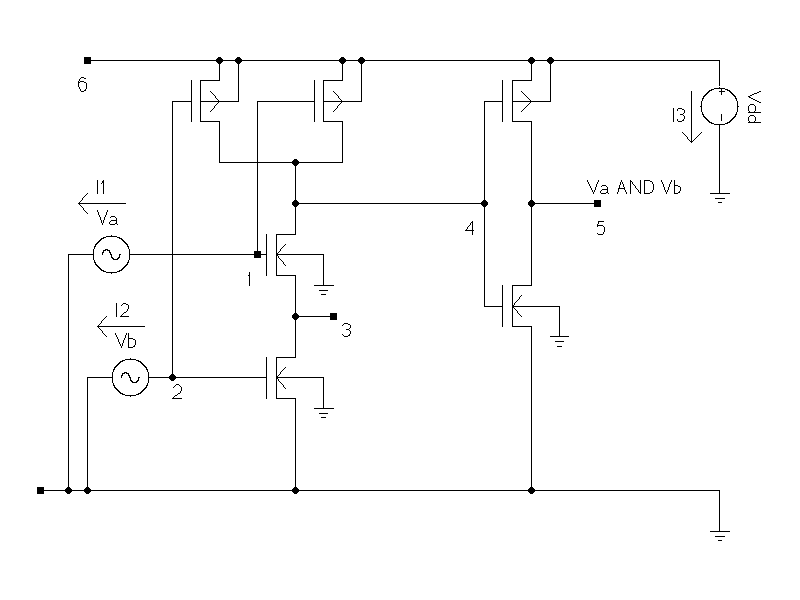
\includegraphics[width=.99\linewidth]{AND_BW.png}
\end{center}
\caption{Schematic of a CMOS AND Gate}\label{fig:and}
\end{figure}

\begin{figure}
\begin{center}
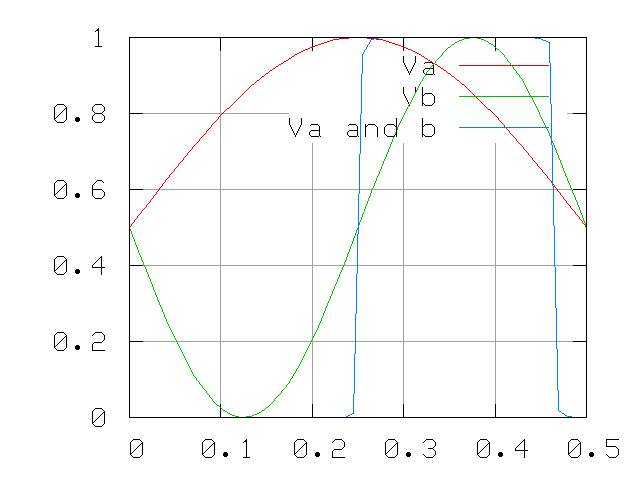
\includegraphics[width=.66\linewidth]{and_output.png}
\end{center}
\caption{Result of the CMOS AND Gate transient simulation}\label{fig:andout}
\end{figure}

%\part*{Appendices}

%\appendix


\subsection{Source Code of the Examples}\label{app:source}

\subsubsection{{\sbn} Files }

\mylistingm{Mvoltagesources}
\mylistingm{Mcurrentsources}
\mylistingm{Mresistors}
\mylistingm{Mnmosfet}
\mylistingm{Mpmosfet}
\mylistingm{Minductors}
\mylistingm{Mcapacitors}

\subsubsection{{\cir} and {\nms} Files}

\mylisting{nmos.cir}
\mylisting{nmos.nms}
\mylisting{pmos.cir}
\mylisting{pmos.nms}
\mylisting{inverter.cir}
\mylisting{inverter.nms}
\mylisting{and.cir}
\mylisting{and.nms}
\mylisting{nmos2.cir}
\mylisting{nmos2.nms}
\mylisting{TLelement.cir}
\mylisting{TLelement.nms}

\subsubsection{Example Parser and Matrix Asembler}

\mylistingm{parseIFF}
\mylistingm{initsystemIFF}
\mylistingm{buildsystemIFF}

\subsubsection{Example Transient Simulations}

\mylistingm{runme}
\mylistingm{runmedaspk}
\mylistingm{plotbynameIFF}
\mylistingm{funres}
\mylistingm{funjac}

 
\end{document}